\documentclass[10pt,journal,compsoc]{IEEEtran}
\usepackage{graphicx}
\usepackage{listings}
\usepackage{float}
\usepackage[spanish]{babel}
\graphicspath{ {D:/OneDrive/TEC/II Semestre 2018/Aseguramiento/Asignación 3/} }
\renewcommand*\contentsname{\'Indice}
\renewcommand\refname{Referencias}


\ifCLASSOPTIONcompsoc
\usepackage[nocompress]{cite}
\else
\usepackage{cite}
\fi

\usepackage{color}

\definecolor{codegreen}{rgb}{0,0.6,0}
\definecolor{codegray}{rgb}{0.5,0.5,0.5}
\definecolor{codepurple}{rgb}{0.58,0,0.82}
\definecolor{backcolour}{rgb}{0.95,0.95,0.92}

\lstdefinestyle{mystyle}{
	backgroundcolor=\color{backcolour},   
	commentstyle=\color{codegreen},
	keywordstyle=\color{magenta},
	numberstyle=\tiny\color{codegray},
	stringstyle=\color{codepurple},
	basicstyle=\footnotesize,
	breakatwhitespace=false,         
	breaklines=true,                 
	captionpos=b,                    
	keepspaces=true,                 
	numbers=left,                    
	numbersep=5pt,                  
	showspaces=false,                
	showstringspaces=false,
	showtabs=false,                  
	tabsize=2
}

\lstset{style=mystyle}

\renewcommand*{\lstlistingname}{Notas}

\hyphenation{op-tical net-works semi-conduc-tor}


\begin{document}
	\title{Asignaci\'on 3 \\ \large Instituto Tecnol\'ogico de Costa Rica \\ Escuela de Ingenier\'ia en Computaci\'on\\ Aseguramiento de la Calidad del Software\\ Prof. Ignacio Trejos Zelaya}
	
	
	\author{Franco~Quiros,~Carnet~2013029890\\ Bryan~Mena,~Carnet~2016112933\\ Pablo~Brenes,~Carnet~2016250460}
	
	\markboth{Asignaci\'on 3,~Lunes~1~, Octubre~2018}%
	{Shell \MakeLowercase{\textit{et al.}}: Asignaci\'on 3}
	\maketitle
	
	\IEEEdisplaynontitleabstractindextext
	
	\IEEEpeerreviewmaketitle
	
	\section{Requerimientos Funcionales}
	\par Para el desarrollo de esta asignación se siguen los requerimientos dados en la especificación de la Asignación 3, además, se mantienen los requerimientos de validación expuestos en la Asignación 2:
	\begin{itemize}
		\item Validación de fechas: Como se menciona en el resumen de la investigación acerca del calendario gregoriano se requiere la validación de la excepción existente en el calendario (Salto del 4 de Octubre de 1582 al 15 de Octubre de 1582).
		\item R8 Validación del año: Se requiere que el año que se esta evaluando en funciones como \textit{bisiesto} sea valido dentro del contexto del programa, esto es: año $\geq$ 1582
	\end{itemize}  

\section{Trabajo Final}
\subsection{Decisiones de Diseño Tomadas}
	\par Para este proyecto es importante mencionar las siguientes decisiones de diseño tomadas por el equipo de trabajo:
	\begin{itemize}
		\item Se modificó el código de la Asignación 2, anteriormente los argumentos del programa los evaluaba el método que estaba siendo utilizado, ahora con la asignación 3 se decidió pasar el parseo de los argumentos a la menú de \textit{\textbf{CLI}} don el fin de beneficiar la alta modularidad y en un futuro hacer más fácil la implementación de una interfaz gráfica de usuario.
		\item Se realizan pequeñas modificaciones al código para el parseo de fechas dado un argumento, esto dada la introducción de un 4 argumento (a parte de año mes y día) para algunas funciones, a raíz de esto además, se añade un atributo a la clase Fechas con el fin de almacenar este nuevo argumento.
		\item Se rediseña la \textbf{\textit{CLI}}, específicamente en la opción de pruebas de archivos, con el fin de evitar la repetición de código se reimplementa esta funcionalidad un poco más acoplada con el menú inicial y no se implementa como un "menú" por aparte como se hizo con la Asignación 2.
		\item Se modifica el método día\textunderscore primero\textunderscore enero para que haga uso del método dia\textunderscore semana agregado en la Asignación 3 con el fin de evitar la repetición de código
	\end{itemize}
\subsection{Pruebas Realizadas}
	\par Para finalizar con el trabajo se realizaron una serie de pruebas para verificar los requerimientos funcionales dados en la especificación:
	
\subsection{Diagrama de Clases}
\begin{figure}[H]
	\centering
	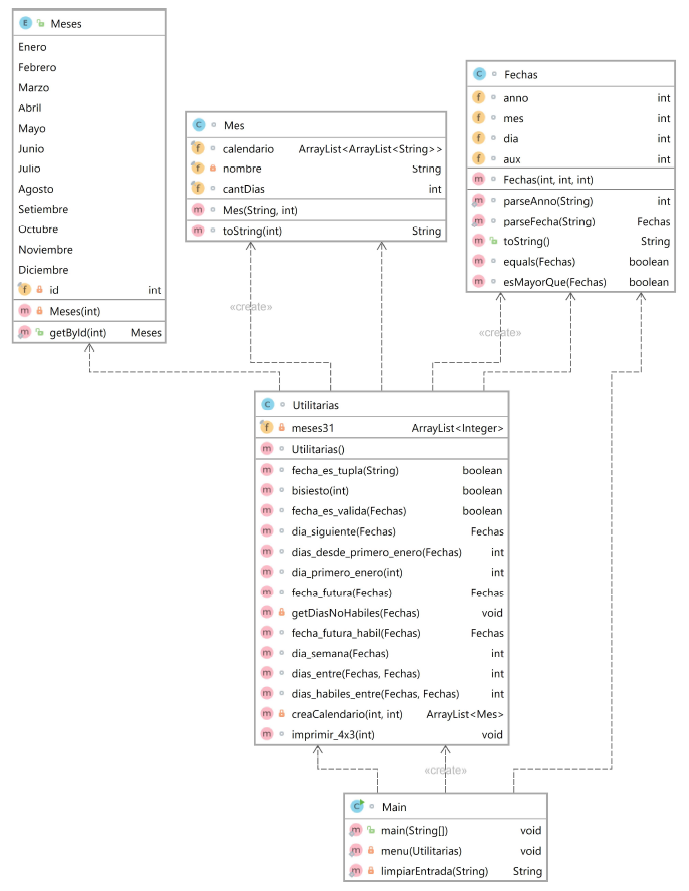
\includegraphics[width=\linewidth]{diagramaClases.png}
	\caption{Diagrama de Clases de la Asignación 3 integrado con la Asignación 2}
\end{figure}
	
\section{Instrucciones de uso}
\par Para el uso del programa mediante la \textbf{\textit{CLI}} se tienen los siguientes comandos:
\begin{itemize}
	\item \textbf{\textit{-h}}: Comando de ayuda muestra una pequeña guía con las funcionalidades del programa
	\item \textbf{\textit{***Requerimientos funcionales Asignación 2***}}
	\item \textbf{\textit{fecha\textunderscore es\textunderscore tupla aaaa mm dd}}: Verificar si una fecha se puede representar en el programa
	\item \textbf{\textit{bisiesto aaaa}}: Retorna verdadero o falso dependiendo si el año dado es bisiesto o no
	\item \textbf{\textit{fecha\textunderscore es\textunderscore valida aaaa mm dd}}: Verifica que la fecha sea valida
	\item \textbf{\textit{dia\textunderscore siguiente aaaa mm dd}}: Retorna la fecha siguiente a la fecha dada
	\item \textbf{\textit{dias\textunderscore desde\textunderscore primero\textunderscore enero aaaa mm dd}}: Retorna la cantidad de días transcurridos entre el primero de enero del año dado a la fecha dada
	\item \textbf{\textit{dia\textunderscore~primero\textunderscore~enero aaaa}}: Retorna el número del día en que cae el 1 de Enero del año dado
	\item \textbf{\textit{imprimir\textunderscore~4x3 aaaa}}: Imprime el calendario en una matriz 4x3 del año dado
	\item \textbf{\textit{***Requerimientos funcionales Asignación 3***}}
	\item \textbf{\textit{fecha\textunderscore futura aaaa mm dd n}}:  Retorna la fecha que está a n días naturales en el futuro
	\item \textbf{\textit{fecha\textunderscore futura\textunderscore habil aaaa mm dd n}}:  Retorna la fecha que está a n días hábiles en el futuro
	\item \textbf{\textit{dia\textunderscore semana aaaa mm dd}}:  Calcula que en que día de la semana se da una determinada fecha
	\item \textbf{\textit{dias\textunderscore entre aaaa mm dd, aaaa mm dd}}:  Retorna la cantidad de días que separa las dos fechas
	\item \textbf{\textit{dias\textunderscore habiles\textunderscore entre aaaa mm dd, aaaa mm dd}}:  Retorna la cantidad de días hábiles que separa las dos fechas
	\item \textbf{\textit{probar\textunderscore archivo nombre}}: Ejecuta cada comando por linea en el archivo de prueba (bajo el mismo formato de los comandos) (Véase \textit{test.txt} incluido en la carpeta de código como un ejemplo del formato para el archivo de pruebas)
	\item \textbf{\textit{salir}}: Termina la ejecución del programa
\end{itemize}
\par Para utilizar el programa se incluye un archivo .jar en la carpeta de Código Fuente llamado ProyectoAseguramiento este archivo puede utilizarse mediante el comando \textit{\textbf{java -jar ProyectoAseguramiento.jar}} en una consola de Windows como se muestra en la figura 6, si se desea compilar los archivos fuentes (disponibles dentro de la subcarpeta dooms de la carpeta Código Fuente) se debe tener en cuenta que todos los archivos pertenecen al paquete \textit{dooms}

\section{Análisis de Resultados}
\par Con un poco más de tiempo y un trabajo más detallado salen a la luz pequeñas pulgas o malas decisiones de diseño que deben ser reparadas antes de integrar la Asignación 2 y la Asignación 3, esto nos muestra que el código está en constante cambio y por más que se revise el código antes de una entrega siempre aparecerán fallos
\newpage
\onecolumn
\appendices
\section{Código de la Asignación 3 integrado con la Asignación 2}
\begin{lstlisting}[language = C, caption = {Se omiten los comentarios en el código con el fin de ahorrar espacio}]
import java.util.ArrayList;

class Utilitarias {
	private final ArrayList<Integer> meses31 = new ArrayList<>();
	Utilitarias(){
		meses31.add(1);
		meses31.add(3);
		meses31.add(5);
		meses31.add(7);
		meses31.add(8);
		meses31.add(10);
		meses31.add(12);
	}
	
	boolean fecha_es_tupla(String argumentos){
		Fechas f = Fechas.parseFecha(argumentos);
		return f != null && fecha_es_valida(f);
	}
	
	boolean bisiesto(int anno){
		if (anno != 0 && anno >= 1582)
			return ((anno % 4 == 0) && ((anno % 100 != 0) || (anno % 400 == 0)));
		else
			return false;
	}
	
	boolean fecha_es_valida(Fechas f){
		if(f != null){
			if(f.mes == 2) {
				return f.anno >= 1582 && f.dia >= 1 && (bisiesto(f.anno) ? f.dia <= 29 : f.dia <= 28);
			}
			else {
				int numDias = meses31.indexOf(f.mes) != -1 ? 31 : 30;
				if (f.anno == 1582 && f.mes == 10) {
					return (f.dia >= 1 && f.dia <= 4) || (f.dia >= 15 && f.dia <= 31);
				}
				else
					return f.anno >= 1582 && f.mes >= 1 && f.mes <= 12 && f.dia >= 1 && f.dia <= numDias;
			}
		}
		else
			return false;
	}
	
	Fechas dia_siguiente(Fechas f){
		if(f != null && fecha_es_valida(f)) {
			int numDias = (f.mes == 2 ? (bisiesto(f.anno) ? 29 : 28) : (meses31.indexOf(f.mes) != -1 ? 31 : 30));
			int dia = f.dia + 1;
			if(f.anno == 1582 && f.mes == 10 && f.dia == 4)
				return new Fechas(1582, 10, 15);
			else if (dia <= numDias)
				return new Fechas(f.anno, f.mes, dia);
			else {
				int mes = f.mes + 1;
				if (mes <= 12)
					return new Fechas(f.anno, mes, 1);
				else
					return new Fechas(f.anno + 1, 1, 1);
			}
		}
		return new Fechas(0, 0, 0); 
	}
	
	int dias_desde_primero_enero(Fechas f){
		if(f != null && fecha_es_valida(f)) {
			int cantDias = 0; 
			for (int i = 1; i < f.mes; i++) {
				if (f.anno == 1582 && i == 10) 
					cantDias += 21;
				else {
					if (i == 2)
						cantDias += bisiesto(f.anno) ? 29 : 28;
					else
						cantDias += meses31.indexOf(i) != -1 ? 31 : 30;
				}
			}
			cantDias += f.dia - 1;
			return cantDias;
		}
		return -1;
	}
		
	int dia_primero_enero(int anno){
		return dia_semana(new Fechas(anno, 1, 1));
	}
	
	Fechas fecha_futura(Fechas f){
		int n = f.aux;
		if(f.anno == 1582 && f.mes == 10)
			n += 10;
		int topeMes = f.mes == 2 ? (bisiesto(f.anno) ? 29 : 28) : (meses31.indexOf(f.mes) != -1 ? 31 : 30);
		int diferenciaMes = topeMes - f.dia;
		while(n > 0){
			if(diferenciaMes > n){
				f.dia += n;
				break;
			}
			else{
				f.dia += diferenciaMes + 1;
				n -= diferenciaMes + 1;
			}
			if (f.mes == 12){
				f.anno++;
				f.mes = 1;
				f.dia = 1;
				diferenciaMes = 30;
				n --;
			}
			else{
				f.mes++;
				f.dia = 1;
				topeMes = f.mes == 2 ? (bisiesto(f.anno) ? 29 : 28) : (meses31.indexOf(f.mes) != -1 ? 31 : 30);
				diferenciaMes = topeMes - f.dia;
			}
		}
		return f;
	}
	
	private void getDiasNoHabiles(Fechas f){
		int diasNoHabiles = 0;
		int diaSemana = dia_semana(f);
		int n = f.aux;
		while(n > 0){
			if(diaSemana == 0){
				diasNoHabiles += 1;
				diaSemana = 1;
			}
			else if(diaSemana == 6){
				diasNoHabiles += 1;
				diaSemana = 0;
			}
			else {
				diasNoHabiles += 1;
				diaSemana += 1;
				n--;
			}
		}
		f.aux = diasNoHabiles;
	}
	
	Fechas fecha_futura_habil(Fechas f){
		if (f == null)
			System.exit(-1);
		getDiasNoHabiles(f);
		f = fecha_futura(f);
		if(dia_semana(f) == 0)
			f = dia_siguiente(f);
		else if(dia_semana(f) == 6){
			f.aux = 2;
			f = fecha_futura(f);
		}
		return f;
	}
	
	int dia_semana(Fechas f){
		int anno = f.anno;
		int mes = f.mes;
		int dia = f.dia;
		int a = (14- mes) / 12;
		anno = anno - a;
		mes = mes + (12 * a) - 2;
		return (dia + anno + anno/4 - anno/100 + anno/400 + (31* mes)/12)%7;
	}
	
	int dias_entre(Fechas f1, Fechas f2){
		Fechas fechaInicio;
		Fechas fechaFin;
		int contador = 0;
		if (f1.esMayorQue(f2)){
			fechaFin = f1;
			fechaInicio = f2;
		}
		else{
			fechaFin = f2;
			fechaInicio = f1;
		}
		while (!fechaInicio.equals(fechaFin)){
			contador += 1;
			fechaInicio = dia_siguiente(fechaInicio);
		}
		return contador;
	}
	
	int dias_habiles_entre(Fechas f1, Fechas f2){
		Fechas fechaInicio;
		Fechas fechaFin;
		int contador = 0;
		if (f1.esMayorQue(f2)){
			fechaFin = f1;
			fechaInicio = f2;
		}
		else{
			fechaFin = f2;
			fechaInicio = f1;
		}
		int diaActual = dia_semana(fechaInicio);
		while (!fechaInicio.equals(fechaFin) && fechaFin.esMayorQue(fechaInicio)){
			if(diaActual == 0){
				fechaInicio = dia_siguiente(fechaInicio);
				diaActual = 1;
			}
			else if(diaActual == 6){
				fechaInicio = dia_siguiente(fechaInicio);
				diaActual = 0;
			}
			else {
				contador += 1;
				fechaInicio = dia_siguiente(fechaInicio);
				diaActual += 1;
			}
		}
		return contador;
	}

	private ArrayList<Mes> creaCalendario(int anno, int dia){
		ArrayList<String> auxiliar = new ArrayList<>();
		ArrayList<Mes> meses = new ArrayList<>();
		auxiliar.add("   D ");
		auxiliar.add("  L ");
		auxiliar.add("  K ");
		auxiliar.add("  M ");
		auxiliar.add("  J ");
		auxiliar.add("  V ");
		auxiliar.add("  S");
		for (int k = 1; k <= 12; k++) {
			int numDias = (k == 2 ? (bisiesto(anno) ? 29 : 28) : (meses31.indexOf(k) != -1 ? 31 : 30));
			String nombreMes = Meses.getById(k).toString();
			ArrayList<String> fila = new ArrayList<>();
			Mes mes = new Mes(nombreMes,numDias);
			mes.calendario.add(auxiliar);
			for (int i = 1; i <= dia; i++)
			fila.add("    ");
			int j = 1;
			while(j <= mes.cantDias){
				if(j == 5 && anno == 1582 && k == 10){
					j = 15;
				}
				if (dia % 7 == 0 && dia != 0){
					mes.calendario.add((ArrayList<String>) fila.clone());
					fila.clear();
				}
				fila.add (( j < 10) ? "   "+j : "  "+j);
				dia += 1;
				j++;
			}
			mes.calendario.add((ArrayList<String>) fila.clone());
			dia %= 7;
			meses.add(mes);
		}
		return meses;
	}

	void imprimir_4x3(int anno){
		int dia = dia_primero_enero(anno);
		ArrayList<Mes> meses = creaCalendario(anno,dia);
		System.out.println("\n\t\t\t\t\t\t\t\t\t\tCalendario " + Integer.toString(anno) + "\n");
		for(int j = 0; j < 12; j+=3){
			String m1;
			String m2;
			String m3;
			for (int i = -1; i<8; i++){
				m1 = meses.get(j).toString(i);
				m2 = meses.get(j+1).toString(i);
				m3 = meses.get(j+2).toString(i);
				System.out.println(m1+"    "+m2+"    "+m3);
			}
		}
	}
}
\end{lstlisting}

\end{document}
